\chapter{Experiments, Results and Analysis}\label{chap:experiments_and_results}

%Present the chapter
In this Chapter the experiment design is presented. Results are shown and an in depth analysis is conducted, including: Energy and distance metrics for measuring the performance
of the proposed methods; A rigorous statistic testing of the proposed methods; A comparison to competing methods in the literature in
order to validate the proposed methods; Finally, a visual inspection of the best predictions
and a comparison against the native conformation.

\section{Design of Experiments}\label{sec:design_of_experiments}

%Present the hardware setup
The experiments were all conducted on a single machine using the same hardware
throughout the full experimentation length. Table~\ref{tab:machine-setup} presents
the machine utilized to run all the experiments. Each run of a prediction method
consists of a serial program that run continually without interruption.
The experiments were run in parallel, limited to at most one running test
per core\footnote{Only physical cores were considered. No virtual (Hyperthreading) core was
involved in the computations.}.
To ensure maximum repeatability the machine had no graphical interface enabled during the course of the experimentation.

\begin{table}[th]
    \centering
    \begin{tabular}{r|l} \hline \hline
        Name & Value \\ \hline \hline
        Operating System & Arch Linux \\ \hline
        Kernel &  Arch Linux Kernel 4.18.16 \\ \hline
        CPU & Intel(R) Core(TM) i5-3570K CPU @ 4.20GHz \\ \hline
        Number of Cores & 4 Physical cores, no hyperthreading cores \\ \hline
        RAM & 16 GB @ 1400 MHz \\ \hline \hline
    \end{tabular}
    \caption{The Machine Setup}
    \label{tab:machine-setup}
\end{table}

The experimentation is separated into two stages. In the first stage the four proposed methods are compared against each other and against a standard \ac{SaDE}. The metrics utilized are the \textit{scorefxn} energy value of the best solution and the \ac{RMSD} associated with the same conformation.
The result was collected over 60 independent runs of each method for each target protein. A graphical analysis is conducted
in order to identify visually the relative performance between the proposed methods.
Considering that a visual analysis is not enough (in this case), a more rigorous numerical
statistic set of test is conducted.
The Shapiro-Wilk~\cite{wilk1968joint} normality test is employed with a confidence level of 5\%, i.e. $\alpha = 0.05$,
to assess the presence (or lack) of a underlying normal distribution. Based on its result, 
a parametric/non-parametric test is employed with a confidence level of $\alpha = 0.05$. Due to the multiple
comparisons involved \v{S}idák's $\alpha$ correction will be utilized~\cite{vsidak1967rectangular}.
The winner (or winners) method(s) will be used in further comparison against the literature.
The processing time for this stage is also analyzed. The time required from the start of the 
initial population generation until the final full atom model is output is measured in seconds.

% Present the protein set
In the second stage of experimentation, 10 independent runs apart from the first stage are used to compare with related works found in the literature. A set of proteins was selected based on previous experiments by other authors. To be able to fully compare the proposed methods with others in the literature only experiments using the same metrics and protein were utilized. This decision limits the number of previous works that can be compared to this one. Furthermore, it also limits the number of times that the proposed methods can be ran. Nevertheless, it provides a solid comparison standard. The metrics utilized are the best scorefxn energy function and the best \ac{RMSD} from all runs, and the mean and standard deviation of the scorefxn energy function of all runs. A direct comparison of the minimum energy and \ac{RMSD} will be used as criterion for comparing the methods. % as well as an unpaired Student T Test.
%
%\textbf{CREIO QUE ESTE PARÁGRAFO DEVA SER REMOVIDO PQ TEM INFOS REDUNDANTES E DIFERENTES DO PARÁGRAFO ANTERIOR. CORRETO?}
%\textcolor{blue}{Não, o primeiro testa utilizadno 60 execuções para comprar os metodos propostos entre si. O segundo utiliza 10 execuções (para manter o padrão com a literatura) para comparar com outros trabalhos. São dois experimentos diferentes com execuões diferentes} 

With this constraints and considerations a set of four proteins was assembled: 1ZDD, 1CRN, 1ENH and 1AIL. Table~\ref{tab:protein-targets} presents some characteristics of the set of proteins chosen as test suit.
The column \textbf{Name} contains the protein identification code as in PDB.
The \textbf{Size} column shows the number of amino acids in the protein.
The \textbf{Backbone Angles} column shows the number of angles in the backbone,
this also has a one to one relation to the number of variables to be optimized
for a given protein. The \textbf{Structure} column holds the secondary structures
present in the protein set represented by $\alpha$-helices or $\beta$-sheets.

\begin{table}[bh]
  \centering
  \begin{tabular}{ l | c | c | c | c }
    \hline \hline
    Name & Size & Backbone Angles & Structure         \\ \hline \hline
    1ZDD & 35   & 105             & $2\alpha$         \\ \hline
    1CRN & 46   & 138             & $2\alpha, 2\beta$ \\ \hline
    1ENH & 54   & 162             & $3\alpha$         \\ \hline
    1AIL & 72   & 216             & $3\alpha$         \\ \hline
    \hline
  \end{tabular}
  \caption{Target proteins and their features}
  \label{tab:protein-targets}
\end{table}

% present each protein
The 1ZDD protein is the smallest one and contains 35 amino acids, amounting
to 105 backbone angles to be optimized. Its structure is very simple consisting
of two $\alpha$-helices that extends all over the backbone except for a small
loop region in the middle that spans over 5 amino acids.
Figure~\ref{fig:1zdd-ss} shows a diagram of the primary sequence, identified as PDF, and the secondary structure, identified as DSSP, of the protein. Due to its size and
secondary structures this protein can be considered the easier of the set.

\begin{figure}[ht]
    \centering
    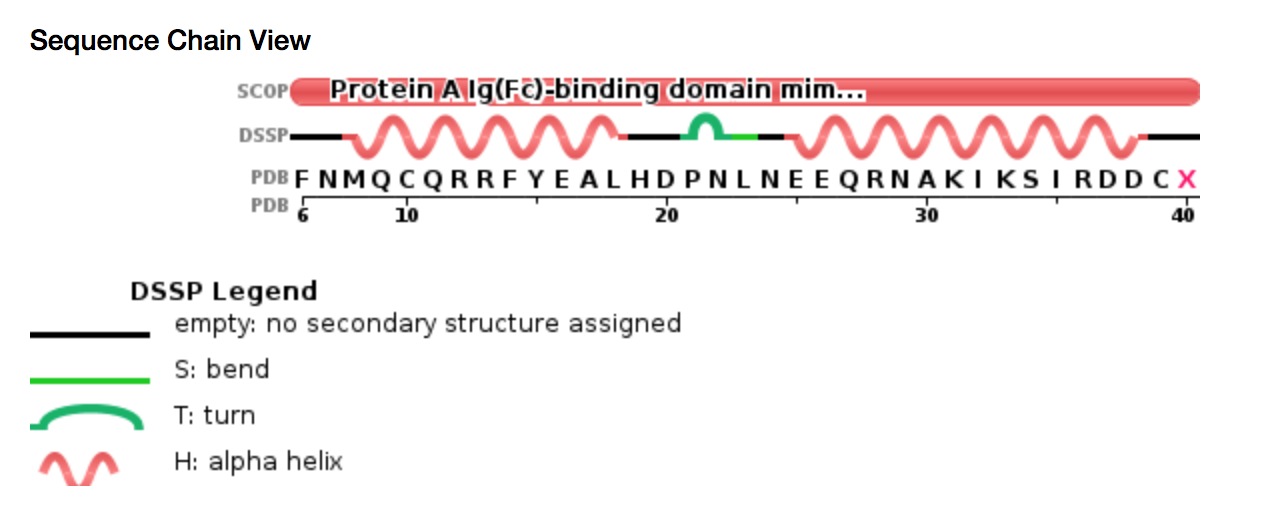
\includegraphics[scale=0.55]{Figuras/1zdd-ss.png}
    \caption{Primary and Secondary Structures of 1ZDD (Source: PSIPRED Server)}
    \label{fig:1zdd-ss}
\end{figure}

The second protein is the 1CRN. It has 46 amino acids and 138 backbone angles
to be optimized. As shown in Figure~\ref{fig:1crn-ss}, the protein has a more
complex structure. It consists of two non-symmetrical $\alpha$-helices separated
by a 5 amino acid loop. At the start of the protein there is a $\beta$-sheet which
matches with another $\beta$-sheet at the last third of the protein. The
final section of the protein forms a coil of 10 residues. Due to
this characteristics this protein can be considered the hardest
target in this set, even though it is the second smallest target.

\begin{figure}[ht]
    \centering
    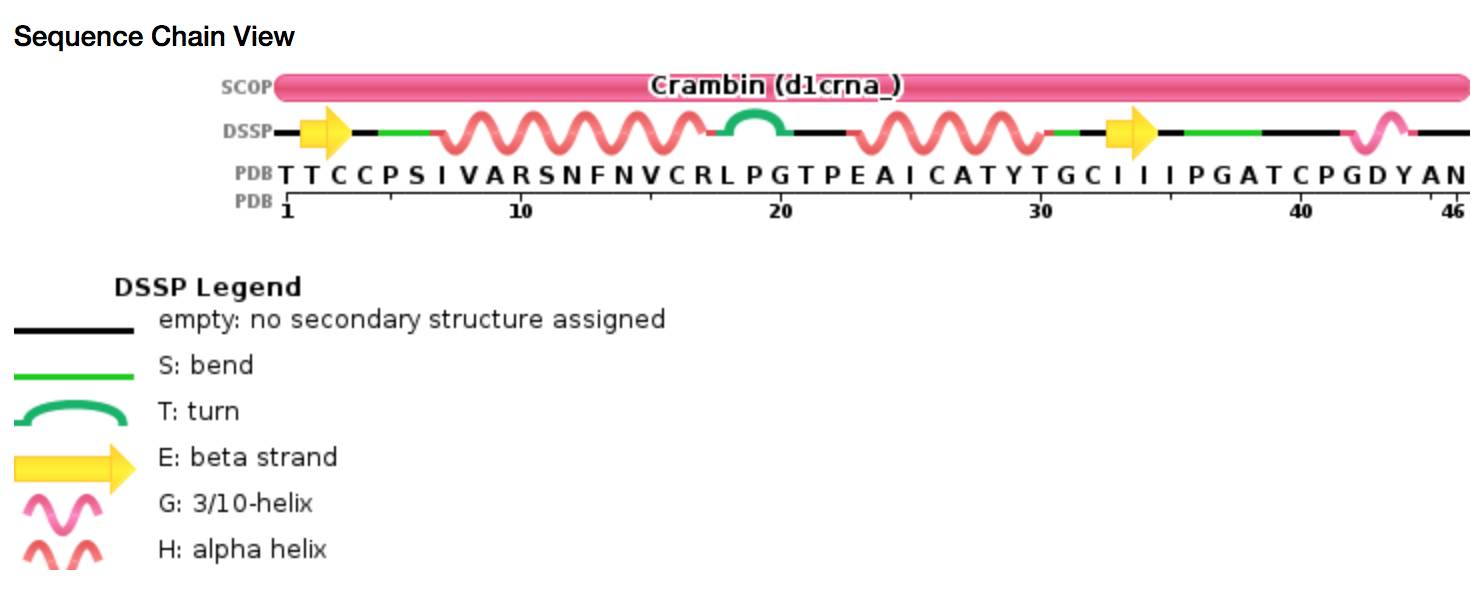
\includegraphics[scale=0.55]{Figuras/1crn-ss.png}
    \caption{Primary and Secondary Structures of 1CRN (Source: PSIPRED Server)}
    \label{fig:1crn-ss}
\end{figure}

The 1ENH and 1AIL proteins are very similar in its structure. The 1ENH has 54 amino acids and 162 backbone torsion angles to be optimized. The 1AIL is the largest protein of this set having 72 amino acids and 216 backbone torsion angles. As can be seen in Figures~\ref{fig:1enh-ss}
and~\ref{fig:1ail-ss} both proteins have 3 $\alpha$-helices spanning the major
portion of the backbone and a turn spanning 5 amino acids between the
first and the second $\alpha$-helices. The 1ENH protein has a coil
of 7 amino acids at it start, meanwhile 1AIL has no coils of significant size.
Both proteins can be considered of similar difficulty. While 1ENH has a bigger
number of coil residues, the 1AIL protein is 18 residues longer, which balances the difficulty of them to be very similar.

\begin{figure}[ht]
    \centering
    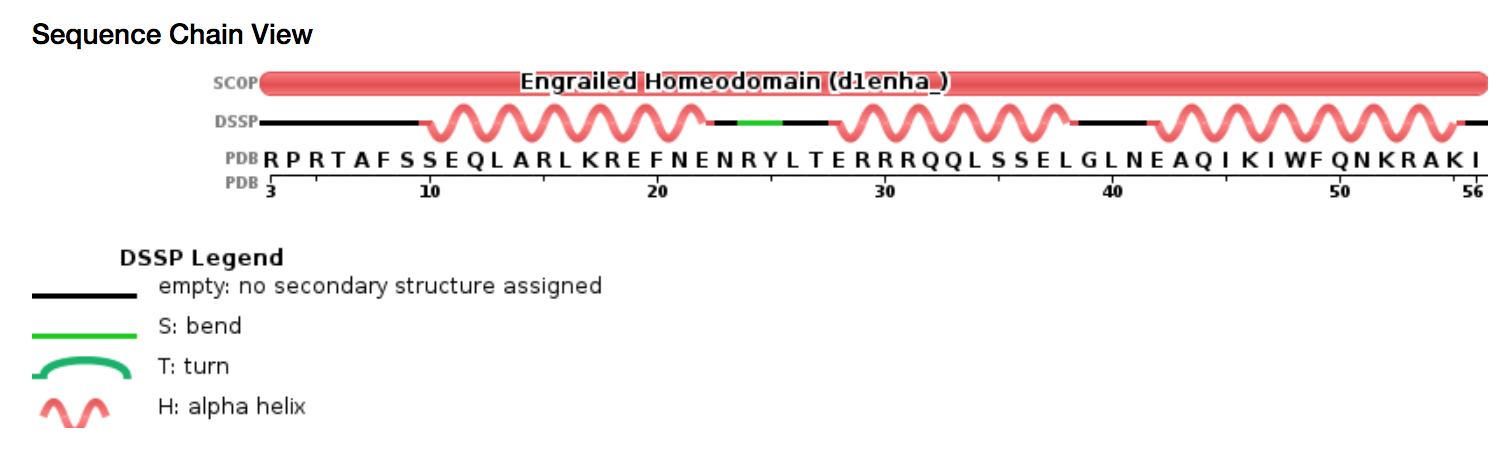
\includegraphics[scale=0.55]{Figuras/1enh-ss.png}
    \caption{Primary and Secondary Structures of 1ENH (Source: PSIPRED Server)}
    \label{fig:1enh-ss}
\end{figure}

\begin{figure}[ht]
    \centering
    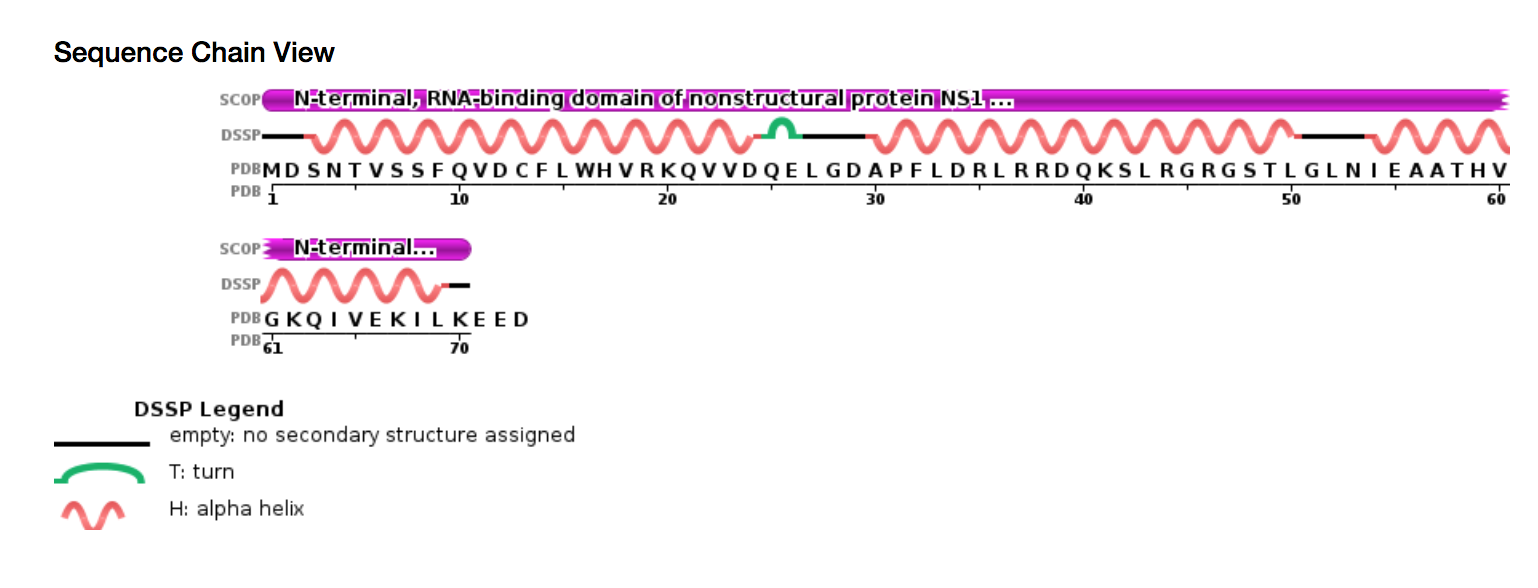
\includegraphics[scale=0.55]{Figuras/1ail-ss.png}
    \caption{Primary and Secondary Structures of 1AIL (Source: PSIPRED Server)}
    \label{fig:1ail-ss}
\end{figure}

% present the four (or six) algorithms
Considering the proposed operators, four combinations of them are possible. The SADE-DE-MC uses \ac{SaDE} with the standard DE set of operators along with MC based fragment insertion. The SADE-MC uses only the MC based fragment insertion without the DE operators. The same applies for the SADE-DE-REMC and for the SADE-REMC, however, instead of a MC sampling method they employ a REMC method.

% Present the parameters
All four proposed methods uses the same parameters. The only difference between them are
the operators available. Table~\ref{tab:parameters} presents the parameters utilized.
The first column shows the name of the parameter and the second column shows the value utilized.
Considering the works in the literature which are comparable with the proposed methods,
a value of 500000 function evaluations was chosen in order to maintain the same number
of function evaluations as used in these works. A separate function evaluation budget
is utilized for the MC and REMC operators, which can spend more than one function evaluation
per operator application. This budget is renewed each time the operator is applied and
discounts from the total function evaluation budged. The value empirically chosen for this budget was 100 function evaluations.
For the generation of the initial pool
of solution vectors the same budget is employed but applied only once using the \textit{score0} energy function. In other words, the MC sampling procedure
applies up to 100 fragment insertions for each initial solution vector.

\begin{table}[ht]
    \centering
    \begin{tabular}{r|l} \hline \hline
        Parameter & Value \\ \hline \hline
        SaDE learning Phase & 50 \\ \hline
        Population Size & 100 \\ \hline
        Function Evaluation Budget & 500000 \\ \hline
        MC/REMC Function Evaluation Budget & 100 \\ \hline \hline
    \end{tabular}
    \caption{Parameters utilized in the proposed methods}
    \label{tab:parameters}
\end{table}

\section{Energy and \ac{RMSD} Analysis}\label{sec:methods-analysis}

% Present the metrics to be utilized
%With the goal of accessing the performance of the proposed methods each method was run 10 times on the protein set and its results recorded. The final output of the prediction can be measured using several different metrics. To allow for a direct comparison with the previous works in the literature the \textit{scorefxn} was used to measure the conformation potential energy and RMSD to measure the error of the prediction compared to the native conformation. \textbf{TEXTO REDUNDANTE VISTO QUE JÁ FOI INSERIDO NA SEÇÃO ANTERIOR.}

%Show the energy and distance table

%\textbf{DE MANEIRA GERAL, CONSIDERANDO TODOS OS RESUTADOS DE TODOS OS EXPERIMENTOS, ACHEI A ANÁLISE ESTATÍSTICA COM RELAÇÃO ÀS SIGNIFICÂNCIAS BEM FRACA. MELHORAR O TEXTO NESTE ASPECTO. VEJA COMENTÁRIO QUE COLOQUEI NA SEÇÃO DO PROJETO DOS EXPERIMENTOS.}

%\textbf{REVEJA TODO O TEXTO ONDE VC MENCIONA 'OVER 60 RUNS'. FICA CHATO TODA HR ESTAR ESCRITO ISTO VISTO QUE VC JA DEIXOU CLARO NA SEÇÃO DO PROTOCOLO DE EXPERIMENTOS QUANTAS FORAM AS EXECUÇÕES.}

%\textbf{NA TABELA 7 SADE-DE É REDUNDANTE PQ O SADE JÁ É O DE. SIMPLIFIQUE NA TABELA E NO TEXTO PARA SOMENTE SADE.}
%\textcolor{blue}{ Eu prefiro deixar SADE-DE, qndo me refiro ao sade eu utilizo SaDE (assim q o artigo original apresenta. SADE-DE eu chamo o experimento q tem o SADE utilizando os operadores do DE. Se eu deixar ele apenas como SADE, então SADE-MC da a entender q tem o DE junto, mas não tem. Creio q do jeito q está agora fica mais claro}

A compilation of the potential energy and the \ac{RMSD} is available in Table~\ref{tab:proposed-methods-results}
for the four proposed methods and for a standard \ac{SaDE} algorithm applied over the four benchmark proteins.
Column \textbf{Protein} shows the PDB code name for the protein. The \textbf{Algorithm} column
shows the methods code name as presented in the previous chapter. The \textbf{Min. Energy} contains
the smallest scorefxn energy found \textbf{over 60 runs}. The \textbf{RMSD} column shows the best \ac{RMSD} between
the predicted conformation of the target protein and its native conformation. Column \textbf{Avg. Energy}
presents the mean and standard deviation of the scorefxn energy. The highlighted values
indicate the smallest value when considering just the absolute value.
% \textbf{NENHUM TESTE ESTATÍSTICO FOI FEITO AQUI?!}

% \textbf{DA TABELA 7, COSIDERE SOMENTE SADE NA ENTRADA ONDE CONTEM SADE-DE. É REDUNDANTE DIZER QUE O SADE USA O DE.}


% Tabela antiga (q eu perdi os dados originais)
% \begin{table}[ht!]
%   \centering
%   \begin{tabular}{ l | l | l | l | r }
%     \hline \hline
% Protein              & Algorithm    & Min. Energy         & RMSD$\alpha$({\AA}) & Avg. Energy             \\ \hline \hline
% \multirow{4}{*}{1ZDD}& SADE-DE-MC   & -62.49              & 2.97              & $-30.44 \pm 27.07$        \\ \cline{2-5}
%                      & SADE-DE-REMC & -70.06              & 1.81              & $-53.17 \pm 11.33$        \\ \cline{2-5}
%                      & SADE-MC      & -80.67              & 1.51              & $\bm{-69.36 \pm 5.50}$    \\ \cline{2-5}
%                      & SADE-REMC    & \textbf{-82.46}     & \textbf{1.16}     & $-68.36 \pm 8.50$         \\ \cline{2-5}
%                      & SADE-DE      & -28.11              & 3.35              & $42.18 \pm 53.02$         \\ \hline \hline
% \multirow{4}{*}{1CRN}& SADE-DE-MC   & -44.02              & 7.80              & $2.31 \pm 55.94$          \\ \cline{2-5}
%                      & SADE-DE-REMC & -31.60              & 5.45              & $3.67 \pm 36.82$          \\ \cline{2-5}
%                      & SADE-MC      & -68.38              & \textbf{5.38}     & $\bm{-45.29 \pm 20.70}$   \\ \cline{2-5}
%                      & SADE-REMC    & \textbf{-82.72}     & 6.08              & $-23.18 \pm 55.94$        \\ \cline{2-5}
%                      & SADE-DE      & 33.72               & 8.36              & $166.45 \pm 82.23$        \\ \hline \hline
% \multirow{4}{*}{1ENH}& SADE-DE-MC   & -112.64             & 4.40              & $-87.63 \pm 15.95$        \\ \cline{2-5}
%                      & SADE-DE-REMC & -113.93             & 3.90              & $-86.12 \pm 30.66$        \\ \cline{2-5}
%                      & SADE-MC      & \textbf{-127.31}    & 4.69              & $\bm{-104.09 \pm 12.06}$  \\ \cline{2-5}
%                      & SADE-REMC    & -125.89             & \textbf{3.23}     & $-98.75 \pm 10.04$        \\ \cline{2-5}
%                      & SADE-DE      & -48.26              & 7.48              & $-21.19 \pm 22.31 $       \\ \hline \hline
% \multirow{4}{*}{1AIL}& SADE-DE-MC   & -126.31             & 7.28              & $-96.70 \pm 22.63$        \\ \cline{2-5}
%                      & SADE-DE-REMC & -149.37             & 6.43              & $-106.08 \pm 31.94$       \\ \cline{2-5}
%                      & SADE-MC      & -142.05             & 7.41              & $-118.39 \pm 13.01$       \\ \cline{2-5}
%                      & SADE-REMC    & \textbf{-159.48}    & \textbf{4.46}     & $\bm{-119.16 \pm 25.01}$  \\ \cline{2-5}
%                      & SADE-DE      & -74.20              & 7.06              & $ -33.00 \pm 27.34$       \\ \hline \hline
%   \end{tabular}
%   \caption{Results from the proposed methods}
%   \label{tab:proposed-methods-results}
% \end{table}

\begin{table}[ht!]
  \centering
  \begin{tabular}{ l | l | l | l | r }
    \hline \hline
Protein               & Algorithm    & Min. Energy      & RMSD$\alpha$ ({\AA}) & Avg. Energy                \\ \hline \hline
\multirow{4}{*}{1ZDD} & SADE-DE      & -52.05           & 2.91                 & $ -28.46 \pm 19.12       $ \\ \cline{2-5}
                      & SADE-DE-MC   & -73.33           & 2.43                 & $ -38.92 \pm 19.18       $ \\ \cline{2-5}
                      & SADE-DE-REMC & -78.19           & 1.58                 & $ -41.81 \pm 20.02       $ \\ \cline{2-5}
                      & SADE-MC      & -81.72           & \textbf{1.25}        & $ \bm{-68.42 \pm 7.44}   $ \\ \cline{2-5}
                      & SADE-REMC    & \textbf{-84.90}  & 1.27                 & $ -66.73 \pm 7.11        $ \\ \hline \hline
\multirow{4}{*}{1CRN} & SADE-DE      & -32.26           & 6.01                 & $ 5.87 \pm 26.70         $ \\ \cline{2-5}
                      & SADE-DE-MC   & -74.64           & 4.60                 & $ -45.34 \pm 16.55       $ \\ \cline{2-5}
                      & SADE-DE-REMC & -82.38           & 4.69                 & $ -47.56 \pm 20.87       $ \\ \cline{2-5}
                      & SADE-MC      & -82.04           & 5.18                 & $ -59.80 \pm 12.68       $ \\ \cline{2-5}
                      & SADE-REMC    & \textbf{-86.18}  & \textbf{3.16}        & $ \bm{-60.58 \pm 10.56}  $ \\ \hline \hline
\multirow{4}{*}{1ENH} & SADE-DE      & -82.68           & 4.73                 & $ -24.60 \pm 60.00       $ \\ \cline{2-5}
                      & SADE-DE-MC   & -128.50          & 3.20                 & $ -101.42 \pm 16.66      $ \\ \cline{2-5}
                      & SADE-DE-REMC & -121.14          & 3.01                 & $ -97.77 \pm 12.64       $ \\ \cline{2-5}
                      & SADE-MC      & -125.15          & \textbf{2.88}        & $ \bm{-107.70 \pm 9.29}  $ \\ \cline{2-5}
                      & SADE-REMC    & \textbf{-129.76} & 3.01                 & $ -105.13 \pm 9.23       $ \\ \hline \hline
\multirow{4}{*}{1AIL} & SADE-DE      & -110.02          & 9.01                 & $ -86.51 \pm 14.12       $ \\ \cline{2-5}
                      & SADE-DE-MC   & -149.32          & 5.39                 & $ -110.10 \pm 19.85      $ \\ \cline{2-5}
                      & SADE-DE-REMC & \textbf{-160.95} & 6.49                 & $ -106.23 \pm 23.46      $ \\ \cline{2-5}
                      & SADE-MC      & -153.09          & 5.78                 & $ -122.62 \pm 13.81      $ \\ \cline{2-5}
                      & SADE-REMC    & -157.31          & \textbf{5.10}        & $ \bm{-126.36 \pm 12.05} $ \\ \hline \hline
  \end{tabular}
  \caption{Results from the proposed methods and SADE-DE aggregated from 60 independent runs.}
  \label{tab:proposed-methods-results}
\end{table}

%Analyze the energy
An inspection on Table~\ref{tab:proposed-methods-results}
shows that SADE-REMC had the best energy for three out of
four proteins, losing only on the 1AIL protein.
On 1AIL, SADE-DE-REMC has the best energy, with SADE-REMC close behind with a difference of
$3.64$ units. SADE-DE, the method with no domain specific operators had the worst
Min. Energy in all four proteins. Looking at the second worst method (relative to the minimum
energy found) and SADE-DE, the distance between them was around 40 energy units, with the
exception of 1ZDD which had 21.28 units. Meanwhile, the amplitude (difference of maximum
and minimum) of the minimum energy for all four proteins was between 12 and 8. This
is a strong indicator of the impact of using domain specific operators.

%On 1ENH, SADE-MC had the best overall energy with SADE-REMC close behind with a difference of less than 3 units. On 1ZDD, the SADE-MC method also had a similar performance to SADE-MC with a difference of less than 2 units. Furthermore, all proposed methods outperformed the standard SaDE method which
%uses no problem domain operators. The methods that used fragment insertion coupled with the standard DE set of operators had results inferior to SADE-MC and SADE-REMC, with the exception
%of SADE-DE-REMC which was able to outperform, when considering only the min. energy, SADE-MC on the 1AIL protein.

% Analyze the distance
Considering the Best \ac{RMSD}, SADE-REMC has the best result on 1AIL and 1CRN. On 1ENH it was
outperformed by SADE-MC by 0.13{\AA} and by 0.02{\AA} on 1ZDD. Again, SADE-DE was outperformed
by all other methods. On 1AIL, it was outperformed by SADE-REMC by 3.91{\AA}. On the other proteins
the gap was relatively smaller, but nevertheless significant when compared to the amplitude
of only the methods using domain specific operators. 

%Considering the Best RMSD, the SADE-REMC had again the best
%results on three out of four target proteins, losing only on the 1CRN protein. On the 1CRN protein SADE-REMC was outperformed by SADE-MC, albeit by less than one unit. As shown for the 1ZDD, 1CRN and 1ENH proteins, the four proposed methods using problem domain information were able to outperform the standard SaDE. As for 1AIL, SaDE had a better RMSD value than
%SADE-DE-MC and SADE-MC. SADE-DE-REMC had an RMSD less than a unit away from SADE-DE, possibly indicating its sub-par performance.

% Analyze the avg energy
% For the average and standard deviation of the energy, SADE-MC and SADE-REMC achieved better or equal results in all proteins.
% For 1CRN it is worth noting a very high standard deviation, indication
% of the hardness of predicting the 1CRN protein, possibly due to a more
% complex energy landscape.
% SADE-DE-MC and SADE-DE-REMC both had a mean energy bigger than zero. On 1ZDD, 1CRN and 1ENH, the SADE-MC and SADE-REMC had statistically the same results and were able to outperform the other methods, as confirmed with an unpaired Student's T-Test. For 1AIL, all four
% proposed methods were statistically equivalent. The standard SaDE method was statistically worse than all four proposed methods, reinforcing the hypothesis that using problem domain information improves PSP.

%An initial analysis of the average and standard deviation of the potential energy obtained for the predictions shows a similar trend as pointed out by the two previous analysis. SADE-REMC and SADE-MC seems to have a similar overall performance which is superior to the other methods. SADE-DE shows a performance inferior than the other methods.
Therefore, based on the data exposed in Table~\ref{tab:proposed-methods-results}, it clear that there is 
a trend towards both SADE-MC and SADE-REMC. These two methods appears to have equivalent performances while
being better than the other proposed methods and the standard SADE-DE. 


% \textbf{INSIRA UMA 'OVERALL ANALYSIS' DA TABELA 7. QUEM/QUAIS FOI/FORAM O/OS MELHOR/ES E PQ? ACHO QUE FALTA UMA ANÁLISE MAIS QUALITATIVA. ESTÁ MUITO DESCRITIVO.}


\begin{figure}[ht]
    \begin{minipage}[b]{0.45\linewidth}
        \centering
        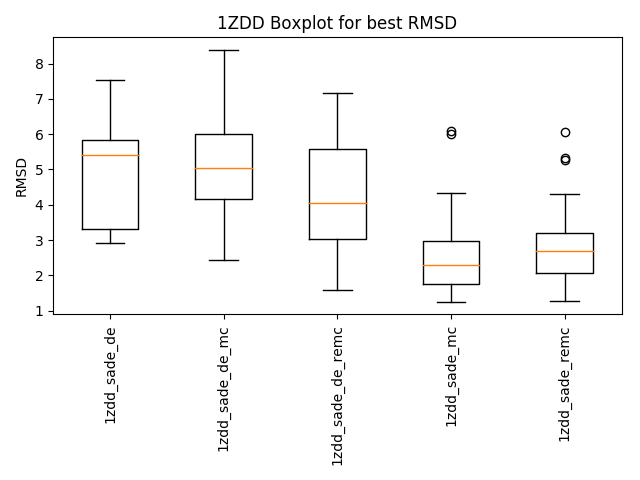
\includegraphics[width=\textwidth]{Figuras/boxplots/1zdd_rmsd_boxplot.png}
        \caption{RMSD boxplot for 1ZDD}
        \label{fig:1zdd-rmsd-boxplot}
    \end{minipage}
    \hspace{0.5cm}
    \begin{minipage}[b]{0.45\linewidth}
        \centering
        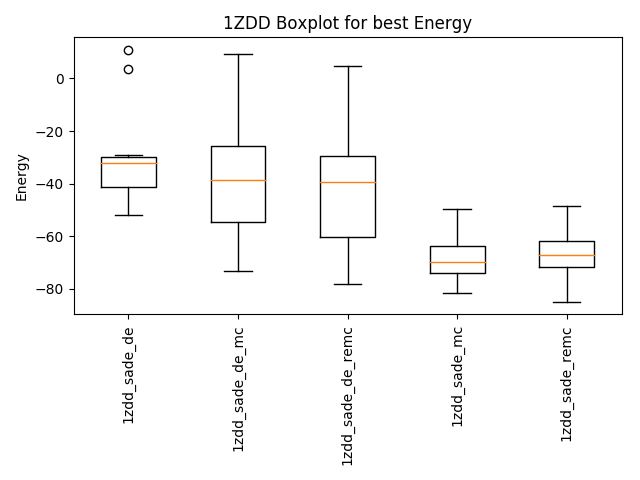
\includegraphics[width=\textwidth]{Figuras/boxplots/1zdd_energy_boxplot.png}
        \caption{Energy boxplot for 1ZDD}
        \label{fig:1zdd-energy-boxplot}
    \end{minipage}
\end{figure}

\begin{figure}[ht]
    \begin{minipage}[b]{0.45\linewidth}
        \centering
        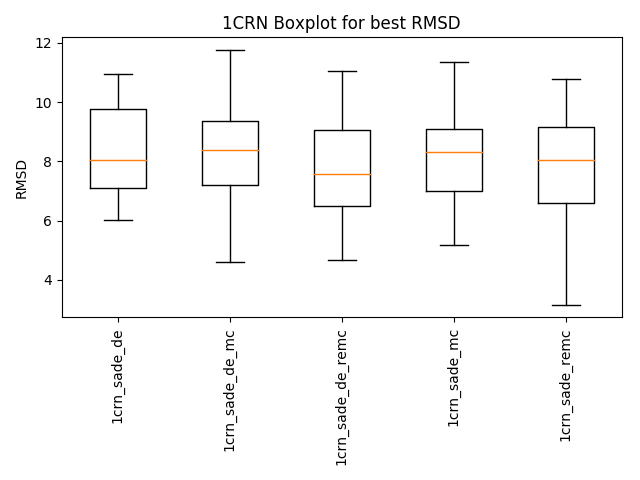
\includegraphics[width=\textwidth]{Figuras/boxplots/1crn_rmsd_boxplot.png}
        \caption{RMSD boxplot for 1CRN}
        \label{fig:1crn-rmsd-boxplot}
    \end{minipage}
    \hspace{0.5cm}
    \begin{minipage}[b]{0.45\linewidth}
        \centering
        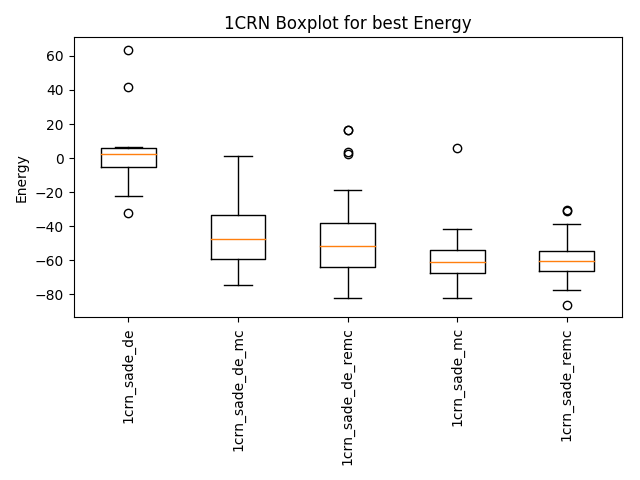
\includegraphics[width=\textwidth]{Figuras/boxplots/1crn_energy_boxplot.png}
        \caption{Energy boxplot for 1CRN}
        \label{fig:1crn-energy-boxplot}
    \end{minipage}
\end{figure}

\begin{figure}[ht]
    \begin{minipage}[b]{0.45\linewidth}
        \centering
        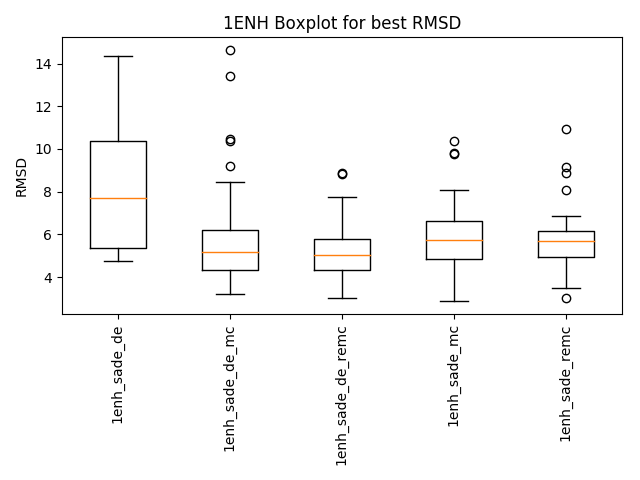
\includegraphics[width=\textwidth]{Figuras/boxplots/1enh_rmsd_boxplot.png}
        \caption{RMSD boxplot for 1ENH}
        \label{fig:1enh-rmsd-boxplot}
    \end{minipage}
    \hspace{0.5cm}
    \begin{minipage}[b]{0.45\linewidth}
        \centering
        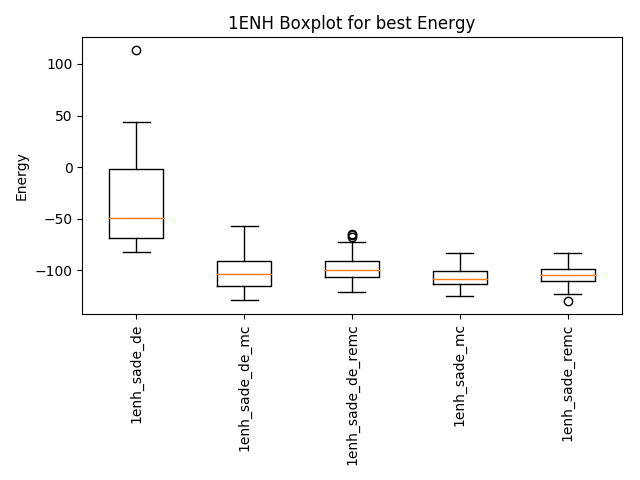
\includegraphics[width=\textwidth]{Figuras/boxplots/1enh_energy_boxplot.png}
        \caption{Energy boxplot for 1ENH}
        \label{fig:1enh-energy-boxplot}
    \end{minipage}
\end{figure}

\begin{figure}[ht]
    \begin{minipage}[b]{0.45\linewidth}
        \centering
        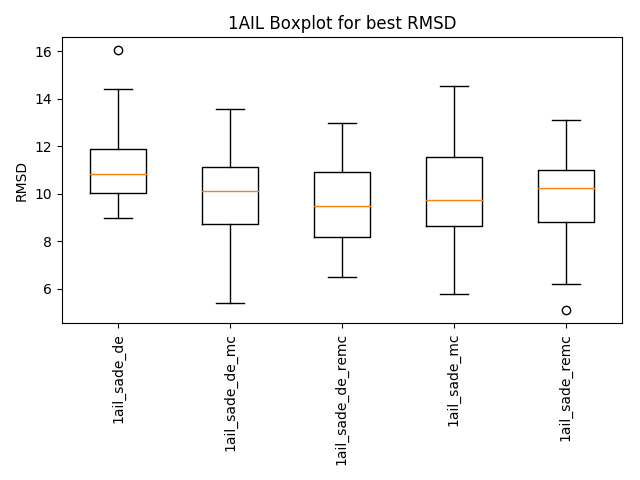
\includegraphics[width=\textwidth]{Figuras/boxplots/1ail_rmsd_boxplot.png}
        \caption{RMSD boxplot for 1AIL}
        \label{fig:1ail-rmsd-boxplot}
    \end{minipage}
    \hspace{0.5cm}
    \begin{minipage}[b]{0.45\linewidth}
        \centering
        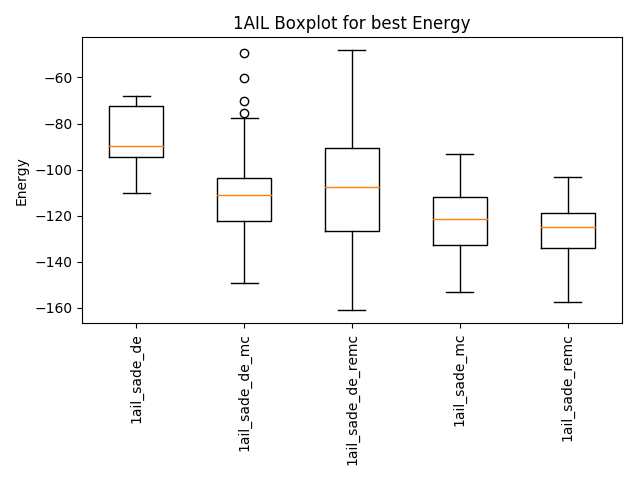
\includegraphics[width=\textwidth]{Figuras/boxplots/1ail_energy_boxplot.png}
        \caption{Energy boxplot for 1AIL}
        \label{fig:1ail-energy-boxplot}
    \end{minipage}
\end{figure}

% \textbf{EM TODOS ESTES BOX-PLOT, SIMPLIFIQUE A ENTRADA DE TEXTO DOS MÉTODOS. NÃO PRECISA INDICAR QUAL É A PROTEÍNA.}
% %
% \textbf{ACHEI A DISPOSIÇÃO DA ANÁLISE ESTRANHA. SUGIRO ANALISAR PRIMEIR O RMSD DE TODAS AS PROTEÍNAS E DEPOIS AS ENERGIAS DE TODAS AS PROTEÍNAS.}
% \textcolor{blue}{A análise  já segue RMSD primeiro e depois a energia.
% Eu acho interessante indicar a proteína
% qndo referencia a figura pro leitor não ter q ir até a figura para ver de qual proteína estou falando.}


Figure~\ref{fig:1zdd-rmsd-boxplot} presents the boxplot for the \ac{RMSD}
of the proposed methods for the 1ZDD protein. Analyzing it it is evident that SADE-MC and
SADE-REMC had better results than the other methods. SADE-DE had the highest overall median.
Figure~\ref{fig:1crn-rmsd-boxplot} shows the same information but for 1CRN. SADE-MC had
the second best \ac{RMSD}, nevertheless its candle overlaps significantly with the others.
The four methods using specific domain operators had very similar candles with a
considerable overlap. SADE-REMC had a prolonged lower quartile, which includes
the predictions with the best \ac{RMSD} in the set.
A noteworthy result in this Figure is that the method with the second lowest median was SADE-DE.
One possible explanation for this is that the fragments utilized can not represent
(or it is under-represented) the 1CRN protein, and as such, it gets stuck in local
minima that does not fully represent the protein.

The boxplot for the \ac{RMSD} of 1ENH is presented in Figure~\ref{fig:1enh-rmsd-boxplot}.
For this protein, SADE-DE-REMC and SADE-DE-REMC have the two lowest medians. A considerable number
of outliers exists above the candles for the four methods using domain specific operators.
The topmost quartile of SADE-DE is also prolonged. This points to the multimodality
of the problem, i.e. the existence of several local minima. In Figure~\ref{fig:1ail-rmsd-boxplot}, the boxplot for the 1AIL protein, SADE-DE had the worst median with the smallest amplitude of the five methods under analysis.
Regardless of the overlap with the other four candles, this is a clear indication
of the relative lower performance of the method.

Figure~\ref{fig:1zdd-energy-boxplot} presents the boxplot with the potential energy
of the proposed methods for the 1ZDD protein. SADE-MC and SADE-REMC had similar candles
which are fully below the median of the other three methods. SADE-DE-MC and SADE-DE-REMC had
similar candles with a considerably high amplitude, ranging from close to the best energy to
positive values. An interesting point is that SADE-DE (with the exception of two outliers)
is fully encompassed in second and third quartiles of SADE-DE-MC and SADE-DE-REMC.
However, as pointed by the lower quartiles of SADE-DE-MC and SADE-DE-REMC, both methods
have a higher potential while SADE-DE gets stuck in a barrier around a energy value of $-40$.
For 1CRN, as shown in Figure~\ref{fig:1crn-energy-boxplot}, a similar scenario occurs.
SADE-MC and SADE-REMC have the best values, followed by SADE-DE-MC and SADE-DE-REMC with
SADE-DE trailing behind. It is worth noting that SADE-DE had its median above zero. This
is a clear indication of poor performance of the method.

For 1ENH the four methods using domain specific operators had very similar results,
as pointed in Figure~\ref{fig:1enh-energy-boxplot}. SADE-MC and SADE-REMC had smaller
amplitudes than the other two methods, albeit for a small margin. SADE-DE had its
upper quartile in the positive energy range. Figure~\ref{fig:1ail-energy-boxplot}
shows the energy boxplot for 1AIL. Here, again, SADE-MC and SADE-REMC had the best two
medians, followed by SADE-DE-REMC and SADE-DE-MC.

The boxplot analysis of \ac{RMSD} and Energy of the four proteins and five methods
shows a tend towards SADE-MC and SADE-REMC in some cases, where in others a mere
visual analysis is inconclusive. Nevertheless, SADE-DE is clearly outmatched.
In other to accurately access the performance of the four proposed methods (using
domain specific operators) further numerical statistical tests are preformed.

In order to utilize statistical tests fist it is
necessary to determine if parametric tests can be utilized. For this, the
Shapiro-Wilk~\footnote{The built-in test available on R was utilized.}
normality test is utilized with an $\alpha = 0.05$.
%\textbf{EXPLICAR O QUE SIGNIFICA PASSAR OU REPROVAR NO TESTE. EXPLIQUE PARA AJUDAR NO ENTENDIMENTO DO QUE SIGNIFICA SER MENOR DO QUE 5\%.} 
The results of the Shapiro-Wilk test are presented in Table~\ref{tab:proposed-methods-shapiro}.
A $p$-$value$ less than $\alpha$ indicates that the protein passed on the test i.e.
it follows a normal distribution and therefore a parametric test can be used.
Otherwise, a non-parametric test must be used. 
The first column presents the protein name
and the second column indicates the method considered. The \ac{RMSD} column shows the
\textit{p-value} for Shapiro-Wilk test applied for the \ac{RMSD}. Column Energy
is analogous as Energy. Values in boldface corresponds to a $p$-$value < \alpha$.
For instance, in the first line in the table SADE-DE with 1ZDD failed
the test for the \ac{RMSD} but passed for the Energy.



\textcolor{red}{
\begin{table}[ht!]
  \centering
  \begin{tabular}{ l | l | l | l }
    \hline \hline
Protein                & Algorithm    & RMSD            & Energy          \\ \hline \hline
\multirow{4}{*}{1ZDD}  & SADE-DE      & 0.2297          & \textbf{0.0327} \\ \cline{2-4}
                       & SADE-DE-MC   & 0.8015          & 0.3044          \\ \cline{2-4}
                       & SADE-DE-REMC & \textbf{0.0697} & 0.0890          \\ \cline{2-4}
                       & SADE-MC      & \textbf{0.0000} & 0.0864          \\ \cline{2-4}
                       & SADE-REMC    & \textbf{0.0029} & 0.9235          \\ \hline \hline
\multirow{4}{*}{1CRN}  & SADE-DE      & 0.2222          & 0.2048          \\ \cline{2-4}
                       & SADE-DE-MC   & 0.8404          & 0.2524          \\ \cline{2-4}
                       & SADE-DE-REMC & 0.2456          & \textbf{0.0001} \\ \cline{2-4}
                       & SADE-MC      & 0.5517          & \textbf{0.0000} \\ \cline{2-4}
                       & SADE-REMC    & 0.1633          & 0.2058          \\ \hline \hline
\multirow{4}{*}{1ENH}  & SADE-DE      & 0.1185          & 0.0749          \\ \cline{2-4}
                       & SADE-DE-MC   & \textbf{0.0000} & \textbf{0.0325} \\ \cline{2-4}
                       & SADE-DE-REMC & \textbf{0.0054} & \textbf{0.0131} \\ \cline{2-4}
                       & SADE-MC      & \textbf{0.0056} & 0.2697          \\ \cline{2-4}
                       & SADE-REMC    & \textbf{0.0002} & 0.5857          \\ \hline \hline
\multirow{4}{*}{1AIL}  & SADE-DE      & 0.1300          & 0.3657          \\ \cline{2-4}
                       & SADE-DE-MC   & 0.5058          & 0.0592          \\ \cline{2-4}
                       & SADE-DE-REMC & 0.3625          & 0.5574          \\ \cline{2-4}
                       & SADE-MC      & 0.3551          & 0.6324          \\ \cline{2-4}
                       & SADE-REMC    & 0.1122          & 0.7365          \\ \hline \hline
  \end{tabular}
  \caption{Shapiro-Wilk tests for the proposed methods}
  \label{tab:proposed-methods-shapiro}
\end{table}
}

Inspecting Table~\ref{tab:proposed-methods-shapiro} it is possible to note that in some cases
the dataset passed the Shapiro-Wilk test. However, it failed in many more. For 1ENH 
the four methods using domain specific operators passed the test for the \ac{RMSD} and
two methods passed for the Energy. For 1CRN two tests passed for the energy and one passed for
1ZDD. On the \ac{RMSD} thee methods passed for 1ZDD. Notably, 1AIL failed for all instances and metrics.
Since there is no clear trend on what methods/metrics passed the tests it can be considered
that the tests do not follow a normal distribution. Therefore, since the underlying distribution
could not be identified a non-parametric test will be utilized.

Assuming a non Gaussian distribution, it is possible to employ the non-parametric two-tailed
Dunn's test for multiple comparisons using \v{S}idák's $\alpha$ correction with $\alpha = 0.05$.
Tables~\ref{tab:1zdd-dunn-energy}-\ref{tab:1ail-dunn-energy} presents these tests for the
energy score for the four proteins. Tables~\ref{tab:1zdd-dunn-rmsd}-\ref{tab:1ail-dunn-rmsd}
presents the tests for the \ac{RMSD} of the same four proteins.


As shown in Table~\ref{tab:1zdd-dunn-energy}, SADE-DE, SADE-DE-REMC and SADE-DE-MC
are statistically equivalent.
A possible reason for this is the simplicity of the protein, in a way that a blind method
can find near optimal solutions due to a smaller/simpler energy landscape.
SADE-MC and SADE-REMC are also statistically equivalent.
Both SADE-MC and SADE-REMC did outperform the other three methods.


\begin{table}[ht!]
  \centering
  \begin{tabular}{ r | l | l | l | l } \cline{2-5}
              & SADE-DE         & SADE-DE-MC      & SADE-DE-REMC    & SADE-MC \\ \hline \hline
SADE-DE-MC    & 0.8549          & -               & -               & -       \\ \hline
SADE-DE-REMC  & 0.5241          & 0.8249          & -               & -       \\ \hline
SADE-MC       & \textbf{0.0000} & \textbf{0.0000} & \textbf{0.0000} & -       \\ \hline
SADE-REMC     & \textbf{0.0000} & \textbf{0.0000} & \textbf{0.0000} & 0.8593  \\ \hline \hline
  \end{tabular}
  \caption{Dunn test with \v{S}idák's $\alpha$ correction for 1ZDD energy scores. Values in bold when $p$ < $\frac{\alpha}{2}$}
  \label{tab:1zdd-dunn-energy}
\end{table}

In Table~\ref{tab:1crn-dunn-energy} a similar result is found, where SADE-MC and SADE-REMC are
statistically equivalent while outperforming the other methods. However, here the complexity
of the problem shows a difference between SADE-DE and the other methods. The blind optimizer
SADE-DE was outperformed by the four proposals of this work. Thus implying that 
the domain specific operators improved the predictive power of the method.


\begin{table}[ht!]
  \centering
  \begin{tabular}{ r | l | l | l | l } \cline{2-5}
              & SADE-DE         & SADE-DE-MC      & SADE-DE-REMC    & SADE-MC     \\ \hline \hline
   SADE-DE-MC & \textbf{0.0046} & -               & -               & -      \\ \hline
 SADE-DE-REMC & \textbf{0.0003} & 0.6540          & -               & -      \\ \hline
      SADE-MC & \textbf{0.0000} & \textbf{0.0000} & \textbf{0.0021} & -      \\ \hline
    SADE-REMC & \textbf{0.0000} & \textbf{0.0000} & \textbf{0.0014} & 0.9977 \\ \hline \hline
  \end{tabular}
  \caption{Dunn test with \v{S}idák's $\alpha$ correction for 1CRN energy scores. Values in bold when $p$ < $\frac{\alpha}{2}$}
  \label{tab:1crn-dunn-energy}
\end{table}

For the 1ENH protein, SADE-DE was outperformed again by the four proposals. SADE-DE-MC was
statistically equivalent to the other three proposed methods. SADE-MC outperformed SADE-DE-REMC
and was equivalent do SADE-REMC. SADE-REMC almost passed the test against SADE-DE-REMC.
Analyzing Figure~\ref{fig:1zdd-energy-boxplot}, it is visible that the candle of
SADE-DE-REMC had a significant overlap of the other three methods, but it was slightly higher.
Nevertheless, all four methods occupied a similar region. Matching this information with
Table~\ref{tab:proposed-methods-results} reveals that the four methods reached the same
plateau, having a very small variance in performance.


\begin{table}[ht!]
  \centering
  \begin{tabular}{ r | l | l | l | l } \cline{2-5}
                 & SADE-DE         & SADE-DE-MC & SADE-DE-REMC    & SADE-MC \\ \hline \hline
   SADE-DE-MC    & \textbf{0.0000} & -          & -               & -       \\ \hline
 SADE-DE-REMC    & \textbf{0.0011} & 0.2041     & -               & -       \\ \hline
      SADE-MC    & \textbf{0.0000} & 0.1370     & \textbf{0.0001} & -       \\ \hline
    SADE-REMC    & \textbf{0.0000} & 0.9401     & 0.0349          & 0.5055  \\ \hline \hline
  \end{tabular}
  \caption{Dunn test with \v{S}idák's $\alpha$ correction for 1ENH energy scores. Values in bold when $p$ < $\frac{\alpha}{2}$}
  \label{tab:1enh-dunn-energy}
\end{table}

For 1AIL a similar scenario as 1CRN happened. SADE-MC and SADE-REMC outperformed the other methods
while being equivalent to each other. SADE-DE-REMC and SADE-DE-MC were statistically equivalent
as well while SADE-DE and SADE-DE-REMC were statistically equivalent. SADE-DE was outperformed by
SADE-DE-MC, SADE-MC and SADE-REMC.


\begin{table}[ht!]
  \centering
  \begin{tabular}{ r | l | l | l | l } \cline{2-5} 
              & SADE-DE & SADE-DE-MC & SADE-DE-REMC & SADE-MC \\ \hline \hline
   SADE-DE-MC & \textbf{0.0166} & -               & -               & -       \\ \hline
 SADE-DE-REMC & 0.0405          & 0.9685          & -               & -       \\ \hline
      SADE-MC & \textbf{0.0000} & \textbf{0.0036} & \textbf{0.0004} & -       \\ \hline
    SADE-REMC & \textbf{0.0000} & \textbf{0.0000} & \textbf{0.0000} & 0.4161  \\ \hline \hline
  \end{tabular}
  \caption{Dunn test with \v{S}idák's $\alpha$ correction for 1AIL energy scores. Values in bold when $p$ < $\frac{\alpha}{2}$}
  \label{tab:1ail-dunn-energy}
\end{table}

Based on this analysis, it is visible that SADE-MC and SADE-REMC have the same predicting
power (measured by the energy) and are superior to the other proposals as well as the blind
optimizer. SADE-DE was outperformed in 13 of the 16 test cases (four methods versus four proteins).
SADE-DE-REMC and SADE-DE-MC had an in-between performance. Therefore, this confirms 
the hypothesis that using domain specific operators for the PSPP improves
prediction performance measured by potential energy.


When analyzing Dunn's test applied to the \ac{RMSD} a different scenario appears. As shown in
Tables~\ref{tab:1zdd-dunn-rmsd}-\ref{tab:1ail-dunn-rmsd}, in only 7 of the 40 tests
(four proteins versus ten comparisons of the methods) there was statistical significance.
Six were for the protein 1ZDD and one for 1ENH. This is a strong indicative
of how hard the problem gets in function of the protein size. On 1ZDD both SADE-MC and
SADE-REMC outperformed the other three methods. On 1ENH SADE-DE-REMC outperformed SADE-DE,
while SADE-DE-REMC came close to being outperformed by SADE-MC. 
The discrepancy between the results measure by the energy and the \ac{RMSD} reveals one of the
main struggles in solving the PSPP using an \textit{ab initio} method. Optimizing
the energy does not necessarily lead to a direct optimization of the \ac{RMSD}, even though
the two are directly correlated. For 1ZDD the hypothesis that using domain specific operators
improves prediction performance (measured by \ac{RMSD}) is thus confirmed. However, the same
was not identified for the remaining three proteins. The most likely cause is due to
poor scaling with the protein size caused by the evergrowing conformational space that has to
be sampled.


\begin{table}[ht!]
  \centering
  \begin{tabular}{ r | l | l | l | l } \cline{2-5}
              & SADE-DE         & SADE-DE-MC      & SADE-DE-REMC    & SADE-MC \\ \hline \hline
SADE-DE-MC    & 0.9886          & -               & -               & -       \\ \hline
SADE-DE-REMC  & 0.8153          & 0.0506          & -               & -       \\ \hline
SADE-MC       & \textbf{0.0001} & \textbf{0.0000} & \textbf{0.0000} & -       \\ \hline
SADE-REMC     & \textbf{0.0012} & \textbf{0.0000} & \textbf{0.0000} & 0.5869  \\ \hline \hline
  \end{tabular}
  \caption{Dunn test with \v{S}idák's $\alpha$ correction for 1ZDD \ac{RMSD}. Values in bold when $p$ < $\frac{\alpha}{2}$}
  \label{tab:1zdd-dunn-rmsd}
\end{table}

\begin{table}[ht!]
  \centering
  \begin{tabular}{ r | l | l | l | l } \cline{2-5}
              & SADE-DE & SADE-DE-MC & SADE-DE-REMC & SADE-MC     \\ \hline \hline
   SADE-DE-MC & 0.9980  & -          & -            & -      \\ \hline
 SADE-DE-REMC & 0.8442  & 0.2217     & -            & -      \\ \hline
      SADE-MC & 0.9968  & 0.9778     & 0.5081       & -      \\ \hline
    SADE-REMC & 0.9657  & 0.6845     & 0.9286       & 0.9220 \\ \hline \hline
  \end{tabular}
  \caption{Dunn test with \v{S}idák's $\alpha$ correction for 1CRN RMSD. Values in bold when $p$ < $\frac{\alpha}{2}$}
  \label{tab:1crn-dunn-rmsd}
\end{table}

\begin{table}[ht!]
  \centering
  \begin{tabular}{ r | l | l | l | l } \cline{2-5}
                 & SADE-DE         & SADE-DE-MC & SADE-DE-REMC    & SADE-MC \\ \hline \hline
   SADE-DE-MC    & 0.0316          & -          & -               & -       \\ \hline \hline
 SADE-DE-REMC    & \textbf{0.0179} & 0.9894     & -               & -       \\ \hline
      SADE-MC    & 0.5132          & 0.0943     & 0.0366          & -       \\ \hline
    SADE-REMC    & 0.3021          & 0.3549     & 0.1793          & 0.9569  \\ \hline \hline
  \end{tabular}
  \caption{Dunn test with \v{S}idák's $\alpha$ correction for 1ENH RMSD. Values in bold when $p$ < $\frac{\alpha}{2}$}
  \label{tab:1enh-dunn-rmsd}
\end{table}

\begin{table}[ht!]
  \centering
  \begin{tabular}{ r | l | l | l | l } \cline{2-5}
              & SADE-DE & SADE-DE-MC & SADE-DE-REMC & SADE-MC \\ \hline
   SADE-DE-MC & 0.2972  & -          & -            & -       \\ \hline
 SADE-DE-REMC & 0.0661  & 0.6949     & -            & -       \\ \hline
      SADE-MC & 0.2595  & 0.9974     & 0.7760       & -       \\ \hline
    SADE-REMC & 0.4835  & 0.9680     & 0.3260       & 0.9421  \\ \hline \hline
  \end{tabular}
  \caption{Dunn test with \v{S}idák's $\alpha$ correction for 1AIL RMSD scores. Values in bold when $p$ < $\frac{\alpha}{2}$}
  \label{tab:1ail-dunn-rmsd}
\end{table}

% Analyze the overall results and conclude
Considering the results obtained, it is possible to conclude that SADE-MC and SADE-REMC had very similar performance and were able to outperform the other proposed methods. Both methods were either equal or better than the other two and the standard \ac{SaDE}. Adding fragment insertion to \ac{SaDE} vastly improved the performance. However, it appears that mixing the DE operator set with fragment insertion has a sub-par performance than using just MC or REMC based fragment insertion under \ac{SaDE} control. One possible explanation for this is that the MC search is going in one direction and DE in other, in such a way that one inhibits the full performance of the other. The underlying mechanism
for this is possibly that DE operates blindingly to the protein structure, possibly trying to make biologically implausible protein conformations.

% \section{Convergence and Diversity Analysis}

% \section{Parameter Analysis and Operator Usage}

% Perhaps?

\section{Processing time}

%\textcolor{red}{\textbf{HORAS? MINUTOS? COLOCAR NA SEÇÃO DO PROTOCOLO DE EXPERIMENTOS QUE O TEMPO TB SERÁ TIRADO E ANALISADO.}}
Table~\ref{tab:processing-times} shows the processing time for each method and protein in seconds.
Each column relates to a Protein and each row to a method. Each cell shows the average processing
time and the standard deviation. The time is counted from the initial population generation
until the algorithm finishes the processing and outputs a full atom conformation.


\begin{table}[ht!]
  \centering
  \begin{tabular}{ r | c | c | c | c } \cline{2-5}
             & 1ZDD                  & 1CRN                  & 1ENH                  & 1AIL                  \\ \hline \hline
SADE-DE      & $ 652.54  \pm 3.29  $ & $ 817.04  \pm 4.07  $ & $ 1092.27 \pm 5.76  $ & $ 1468.05 \pm 10.35 $ \\ \hline
SADE-DE-MC   & $ 674.94  \pm 33.25 $ & $ 955.79  \pm 38.61 $ & $ 1218.09 \pm 59.15 $ & $ 1699.88 \pm 77.13 $ \\ \hline
SADE-DE-REMC & $ 532.41  \pm 8.29  $ & $ 720.36  \pm 13.90 $ & $ 906.96  \pm 21.41 $ & $ 1229.20 \pm 38.15 $ \\ \hline
SADE-MC      & $ 463.91  \pm 17.62 $ & $ 756.96  \pm 47.22 $ & $ 914.89  \pm 62.68 $ & $ 1345.86 \pm 93.59 $ \\ \hline
SADE-REMC    & $ 364.97  \pm 9.48  $ & $ 565.72  \pm 12.49 $ & $ 680.94  \pm 20.52 $ & $ 1012.00 \pm 31.21 $ \\ \hline \hline
%     & SADE-DE              & SADE-DE-MC           & SADE-DE-REMC         & SADE-MC              & SADE-REMC             \\ \hline \hline
%1ZDD & $652.54 \pm 3.29 $   & $674.94 \pm 33.25 $  & $532.41 \pm 8.29 $   & $463.91 \pm 17.62 $  & $364.97 \pm 9.48 $    \\ \hline
%1CRN & $817.04 \pm 4.07 $   & $955.79 \pm 38.61 $  & $720.36 \pm 13.90 $  & $756.96 \pm 47.22 $  & $565.72 \pm 12.49 $   \\ \hline
%1ENH & $ 1092.27 \pm 5.76$  & $ 1218.09 \pm 59.15$ & $ 906.96 \pm 21.41$  & $ 914.89 \pm 62.68$  & $ 680.94 \pm 20.52$   \\ \hline
%1AIL & $1468.05 \pm 10.35 $ & $1699.88 \pm 77.13 $ & $1229.20 \pm 38.15 $ & $1345.86 \pm 93.59 $ & $1012.00 \pm 31.21 $  \\ \hline \hline
  \end{tabular}
  \caption{Processing time of each method in each protein in seconds}
  \label{tab:processing-times}
\end{table}

The blind optimizer SADE-DE is the method with the smaller standard deviations in processing time.
This is mainly due to the fact that even if different operators are chosen, there is little difference
in processing power requirements. SADE-DE is also the second slowest method. The slowest method
is SADE-DE-MC. The extra cost relative to SADE-DE is due to extra time spent inside the Rosetta lib,
mostly with memory management and instantiating objects. The (relatively high) standard deviation
is a direct consequence of using Monte Carlo and the Differential Operators together. The
MC operator can spent up to 100 function evaluations in a single operator calls. This process
happens inside Rosetta and it is very optimized. However, each operator call that calls MC
has a significant overhead. Thus, if the maximum function evaluation budget is spent at once,
there will be a speedup. However, if few function evaluation are spent then the overhead quickly
mounts up, which in turn slows down the method.


The two methods SADE-MC and SADE-REMC are faster than the two variations using the DE operators
due to the more optimized operators that are utilized. The fragment insertion is managed by
Rosetta, which is implemented in Fortran and C++. The DE operators are implemented in Python 3.5,
making it significantly slower. Since SADE-MC and SADE-REMC manipulates the proteins only with 
the Rosetta code, it is inherently faster.


An interesting aspect to note is that SADE-REMC is faster than SADE-MC and that SADE-DE-REMC is
faster than SADE-DE-MC. This happens because each call to the Monte Carlo operator in SADE-MC
has to reinitialize the objects responsible by manipulating the conformations. Meanwhile,
in REMC this behavior is not required. In fact, the non re-initialization of the Pose objects is the mechanism by which the Replica Exchange occurs. This removes much of the overhead,
making the methods using REMC faster than the counter-parts using MC instead.


\section{Comparison with Competing Methods}

To validate the proposals the two top performing methods, i.e. SADE-MC and SADE-REMC, were taken to be compared to other methods found in the literature. In order to provide a fair and direct comparison, some constraints were imposed. Firstly, the energy function being optimized must be the same, i.e. the Rosetta scorefxn. Secondly, the protein set must fully match. These constraints allows to direct compare the performance of the methods via the energy function, since they are the same. This is strictly from a optimization point of view. To compare from the PSP perspective, the \ac{RMSD} is used, which requires the same protein set
to be used to be able to provide a fair comparison.

Three works were found in the literature matching these constraints. The first being the work of~\cite{narloch2017protein} where the authors explored the use of a Cascading Differential Evolution, were different operators were used during different arbitrary set stages. This work will be identified as DE$_{C_1}$ and DE$_{C_2}$. In~\cite{borguesan2015apl} the authors presented a PSO and GA algorithms using statistical data from the dihedral angle distribution based on secondary structure and amino acid.
This information, called APL (Angle Probability List), was used to generate random angles and to perturbate new ones using more biologically plausible torsion angles. Only the GA algorithm with APL will be considered, since it outperform PSO. It will be named GA-APL.
In~\cite{silva2018multistage} the authors utilized a Multistage Simulated Annealing algorithm, where in each stage a different set
of operators and energy function is utilized. This work will be referenced as MSA. The results from these works and the two top performing proposed works are available in Table~\ref{tab:literature-compatison}. The first column presents the name
of the 4 protein used as benchmarks. The Second column presents the methods name.
The column Min. Energy shows the minimum energy obtained from 10 executions
of the method, while the column \ac{RMSD} shows the minimum \ac{RMSD}. The column
Avg. Energy shows the average and the standard deviation of the energy based
on the 10 runs of the algorithm. Both this column and the Min Energy column
are based on the scorefxn energy score.
As shown in Table~\ref{tab:proposed-methods-shapiro}, the underlying distribution of the proposed methods
is not Gaussian, which lead to the use of non-parametric tests in Section~\ref{sec:methods-analysis}.
Because of this, no statistical test can be used in this section since the only available information
are the Mean and Standard Deviation.
Consequently, the analysis can be only conducted based on these two values.



\begin{table}[ht!]
  \centering
  \begin{tabular}{ l | l | l | l | l }
    \hline \hline
Protein              & Algorithm    & Min. Energy         & RMSD$\alpha$({\AA}) & Avg. Energy             \\ \hline \hline
\multirow{6}{*}{1ZDD}& DE$_{C_1}   $& 54.27               & 7.67              & $82.97\pm15.49     $      \\ \cline{2-5}
                     & DE$_{C_2}   $& 65.77               & 9.42              & $82.76\pm9.22      $      \\ \cline{2-5}
                     & GA-APL       & -40.40              & 10.9              & $-36.20\pm2.60$           \\ \cline{2-5}
                     & MSA          & -62.99              & 2.62              & $-48.96\pm7.77$           \\ \cline{2-5}
                     & SADE-MC      & -80.67              & 1.51              & $\bm{-69.36 \pm 5.50}$    \\ \cline{2-5}
                     & SADE-REMC    & \textbf{-82.46}     & \textbf{1.16}     & $-68.36 \pm 8.50$         \\ \hline \hline
\multirow{6}{*}{1CRN}& DE$_{C_1}   $& 82.86               & 21.56             & $126.95\pm25.98    $      \\ \cline{2-5}
                     & DE$_{C_2}   $& 72.48               & 15.44             & $109.08\pm22.96  $        \\ \cline{2-5}
                     & GA-APL       & -22.70              & 5.8               & $-18.20\pm2.9$            \\ \cline{2-5}
                     & MSA          & -76.93              & 6.96              & $\bm{-54.01\pm17.30}$     \\ \cline{2-5}
                     & SADE-MC      & -68.38              & \textbf{5.38}     & $-45.29 \pm 20.70$        \\ \cline{2-5}
                     & SADE-REMC    & \textbf{-82.72}     & 6.08              & $-23.18 \pm 55.94$        \\ \hline \hline
\multirow{6}{*}{1ENH}& DE$_{C_1}   $& 294.25              & 14.72             & $372.11\pm52.05    $      \\ \cline{2-5}
                     & DE$_{C_2}   $& 255.54              & 19.28             & $320.38\pm41.06    $      \\ \cline{2-5}
                     & GA-APL       & -56.08              & 14.99             & $-51.52\pm1.94$           \\ \cline{2-5}
                     & MSA          & -95.86              & 5.70              & $-80.75\pm8.48$           \\ \cline{2-5}
                     & SADE-MC      & \textbf{-127.31}    & 4.69              & $\bm{-104.09 \pm 12.06}$  \\ \cline{2-5}
                     & SADE-REMC    & -125.89             & \textbf{3.23}     & $-98.75 \pm 10.04$        \\ \hline \hline
\multirow{6}{*}{1AIL}& DE$_{C_1}   $& 357.84              & 25.00             & $440.63\pm58.11    $      \\ \cline{2-5}
                     & DE$_{C_2}   $& 332.54              & 16.88             & $411.81\pm56.84    $      \\ \cline{2-5}
                     & GA-APL       & -75.07              & 12.34             & $-71.08\pm3.35$           \\ \cline{2-5}
                     & MSA          & -128.55             & 8.27              & $-117.54\pm10.28$         \\ \cline{2-5}
                     & SADE-MC      & -142.05             & 7.41              & $-118.39 \pm 13.01$       \\ \cline{2-5}
                     & SADE-REMC    & \textbf{-159.48}    & \textbf{4.46}     & $\bm{-119.16 \pm 25.01}$  \\ \hline \hline
  \end{tabular}
  \caption{Results obtained}
  \label{tab:literature-compatison}
\end{table}

With the results presented in Table~\ref{tab:literature-compatison} it is possible to compare the proposed methods to the literature.
For 1ZDD both SADE-MC and SADE-REMC have a significant overlap of the mean and standard deviations, with
no apparent difference in performance. The mean energy of these two methods is about 20 units
better (smaller) than MSA and 25 than GA-APL. A strong indicative that the two proposed methods outperformed
the other competing methods. Against DE$_{C1}$ and DE$_{c2}$ the difference if bigger than 100 units.
Considering the Min. Energy and the RMSD, SADE-REMC had better values than SADE-MC, which in turn had
best values than the other methods.

%For 1ZDD both proposed methods are statistically equivalent between them and better than MSA, GA-APL and both Cascading DE when considering the mean and standard deviation. When competing the RMSD and the Min. Energy the two proposed methods outperforms the other methods from the literature.

For the 1CRN protein, initially it is possible to notice that SADE-REMC had the best
min. energy followed by MSA and then SADE-MC. For the \ac{RMSD}, SADE-MC had the best result followed by GA-APL
and then SADE-REMC with a different of 0.28{\AA}. When analyzing the mean energy MSA had the smallest mean.
Nevertheless, there is a considerable overlap between the means and standard deviations if MSA and SADE-MC. 
Furthermore, considering the Min. Energy for SADE-REMC, its mean and standard deviation, it becomes
evident how spread the performance was, leading to an overlap with SADE-MC and MSA.
A conclusion from this is that in this case, considering the sample at hand, MSA had a more consistent
performance, while SADE-MC and specially SADE-REMC were able to achieve better results at the cost of
a higher variance.

%However, due to a high standard deviation, both proposed methods and MSA are statistically equal.
%The lack of a clear winner for this protein is another indicative of its complexity.

The 1ENH protein presented a very similar min energy for the two proposed methods, which had better values than the competing methods. Analyzing the \ac{RMSD}, SADE-REMC and SADE-MC achieved better results than MSA and the other methods.
The performance of SADE-MC and SADE-REMC the means and standard deviations are close and present
a considerable overlap. Comparing SADE-MC and MSA, the closest competitor so far, there is a difference of
almost 25 units between the means and a difference of 18 units between SADE-REMC and MSA.

%When considering the average energy, both proposed methods were statistically
%better than MSA, which proved to be the closest
%competitor so far.

The 1AIL protein possibly presents the bigger differences between the
proposed methods and the ones from the literature. 
The SADE-REMC had a difference of 17.43 REU (Rosetta Energy
Units) compared to SADE-MC and even more for the other methods.
For the \ac{RMSD}, the difference between SADE-REMC and SADE-MC was of 2.95 {\AA} and for MSA of 3.81 {\AA}.
%However, when considering the average energy, the two proposed methods and MSA were
%statistically equivalents
The means of MSA, SADE-MC and SADE-REMC have a difference of less than 2 units. However, the standard
deviation of SADE-REMC is about two and a half times bigger than MSA. This correlates to
SADE-REMC having the best energy and \ac{RMSD} despite the same mean as the other two methods.

Overall, when considering the minimum energy and \ac{RMSD}, the two proposed methods were able to outperform the other competing methods from the literature.
Considering the mean, MSA had the same results as the two proposed methods on 1AIL. For 1CRN, MSA
had a better mean. However, despite this, SADE-REMC and SADE-MC were able to achieve the better energies
and lowest \ac{RMSD} for all four proteins.
The unavailability of sufficient information on the tests in the literature
prevented a strong and rigorous statistical test. Nonetheless, there is a strong indication that
the hypothesis that online parameter control improves upon methods with no parameter control is true.
Moreover, the same can be said about the hypothesis that a hybrid method improves the prediction
power.


\section{GDT-TS and TM-Score metrics}

%Due to limitations in the availability of works using the TM-Score and/or the GDT-TS metrics on the same target proteins, it was only possible to use the RMSD in order to validate this work against other works in the literature. Nevertheless, with the goal to 

This section provides an in depth analysis of the results obtained in this work using the GDT-TS and the TM-Score metrics of the predicted proteins. The results can also be used by other works to compare against our own using these metrics. Tables~\ref{metrics-gdt-ts} and~\ref{metrics-tm-score} present for the two best proposed methods, SADE-MC and SADE-REMC, their respective GDT-TS and TM-Score. Both tables follows the same format. The first column presents the protein name. The second and third column
presents the data for SADE-MC and SADE-REMC respectively. The data shown is the
best score in parenthesis, followed by the average and the standard deviation.

%%%%%%%%%%%%%%%%%%%%%%%%%%%%%%
\begin{table}[ht!]
  \centering
  \begin{tabular}{ l | l | l }
    \hline \hline
\multirow{2}{*}{Protein}& \multicolumn{1}{c|}{SADE-MC}      & \multicolumn{1}{c}{SADE-REMC}       \\ \cline{2-3}
                        & $(Best) Avg \pm Std Dev $ & $(Best) Avg \pm Std Dev$  \\ \hline \hline
\multirow{1}{*}{1ZDD}   & $(0.860) 0.779 \pm 0.072$ & $(0.860) 0.762 \pm 0.066$ \\ \hline
\multirow{1}{*}{1CRN}   & $(0.543) 0.422 \pm 0.057$ & $(0.462) 0.405 \pm 0.047$ \\ \hline
\multirow{1}{*}{1ENH}   & $(0.463) 0.414 \pm 0.036$ & $(0.463) 0.390 \pm 0.037$ \\ \hline
\multirow{1}{*}{1AIL}   & $(0.407) 0.342 \pm 0.031$ & $(0.449) 0.365 \pm 0.039$ \\ \hline
    \hline \hline
  \end{tabular}
  \caption{Results showing the GDT-TS metric}
  \label{metrics-gdt-ts}
\end{table}

\begin{table}[ht!]
  \centering
  \begin{tabular}{ l | l | l }
    \hline \hline
\multirow{2}{*}{Protein}& \multicolumn{1}{c|}{SADE-MC} & \multicolumn{1}{c}{SADE-REMC}  \\ \cline{2-3}
                      & $(Best) Avg \pm Std Dev $ & $(Best) Avg \pm Std Dev$  \\ \hline \hline
\multirow{1}{*}{1ZDD} & $(0.658) 0.547 \pm 0.091$ & $(0.666) 0.542 \pm 0.085$ \\ \hline
\multirow{1}{*}{1CRN} & $(0.393) 0.288 \pm 0.041$ & $(0.295) 0.261 \pm 0.033$ \\ \hline
\multirow{1}{*}{1ENH} & $(0.288) 0.254 \pm 0.022$ & $(0.292) 0.237 \pm 0.025$ \\ \hline
\multirow{1}{*}{1AIL} & $(0.338) 0.281 \pm 0.030$ & $(0.440) 0.298 \pm 0.051$ \\
    \hline \hline
  \end{tabular}
  \caption{Results showing the TM-Score metric}
  \label{metrics-tm-score}
\end{table}

%%%%%%%%%%%%%%%%%%%%%%%%%%%%%%

For the 1ZDD protein, the mean value of the predictions was above 0.5 for GDT-TS and TM-Score for the two methods, meaning that both proposals were able to achieve the same overall fold. Furthermore, for GDT-TS a value bigger than 0.8 strongly indicates that a near native conformation is found. The GDT-TS values for 1CRN and 1ENH protein are close to 0.4 indicating that both methods were
close to finding the same fold to their respective native conformations. The TM-Score for 1CRN, 1ENH and 1AIL proteins had mean values ranging from $0.237$ to $0.298$. When considering this metric, it indicates that the algorithm started to converge but did not arrive quite at the same fold. Considering the Best values, 1AIL for SADE-REMC and 1CRN for SADE-MC had values around $0.4$ which indicates that on some runs the algorithm was close to finding the same overall near native fold.

In hands on this information, a different conclusion is possible when considering only \ac{RMSD}. Considering GDT-TS and specially the TM-Score it is more evident how much room for improvement there still is. The results strongly indicate that the methods performance falls as the number of amino acids in the protein grows. While this is expected, since the number of variables (and thus the search space) increases as the number of amino acids grows, it is more evident on the GDT-TS and TM-Score than when looking only on the \ac{RMSD}. In fact, 1AIL and 1ENH proteins had better results than 1CRN when considering the \ac{RMSD}. However, the GDT-TS and TM-Score metrics show otherwise.

Another aspect is that the GDT-TS and TM-Score metrics roughly agreed
on the results. For some instances, however, they did not. SADE-MC is
pointed to have a better performance on 1AIL than on 1ENH when
considering the TM-Score, however, GDT-TS indicates the opposite.
The most likely cause for this is how different the metrics
measure the difference of each conformation. Furthermore, TM-Score seems to be a metric harder to increase than GDT-TS, as can be seen in Tables~\ref{metrics-gdt-ts} and~\ref{metrics-tm-score}. Both the TM-Score and GDT-TS agree on the overall performance, but for all cases the GDT-TS was higher.

\section{Visual Representation of the Predictions}

With the goal of validating the predictor, the best conformations found by SADE-REMC were selected for a visual analysis. While SADE-MC and SADE-REMC were statistically equivalent, SADE-REMC had the predictions with the smallest \ac{RMSD} in 3 out of 4 proteins. For this reason it was selected to be visually inspected. The predicted conformations were superimposed over the native ones with the goal of providing a clear comparison. Figure~\ref{fig:visual-comparison} contains the 4 proteins utilized in this experiment. In cyan (or the light color) are the predicted conformations and in red (darker color) are the native conformations.

\begin{figure}[ht]
    \centering
    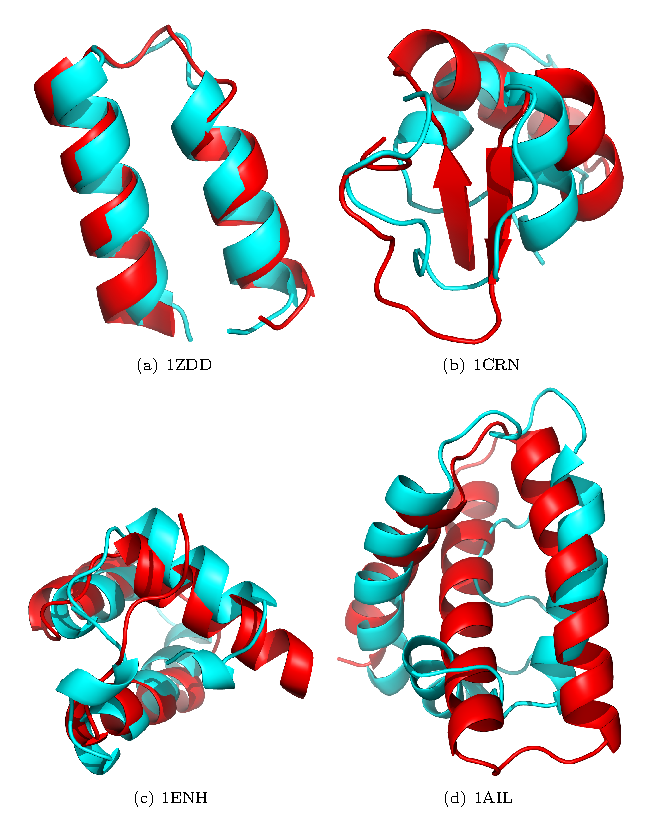
\includegraphics{Figuras/visual_comparison_image.pdf}
    \caption{Predicted Proteins (cyan, lighter) compared to the Native conformations (red, darker)
    (Created with PyMOL)}
    \label{fig:visual-comparison}
\end{figure}


As presented in Figure~\ref{fig:visual-comparison}(a) it is possible to notice that the predicted conformation closely matched the native conformation. Considering that the native conformation is also only a (very close) approximation of the real protein, the \ac{RMSD} of 1.16 can be considered as a near native prediction. 

Figure~\ref{fig:visual-comparison}(b) shows the 1CRN protein, which can be considered the hardest target of this work. This can be confirmed by visual inspection. When compared to the other 3 proteins, 1CRN is visibly more different than the others. Nevertheless, by following along the two backbones (the native and predicted) it is possible to notice that the overall fold of the protein was correctly predicted. One of the main errors of the prediction was the left-most $\alpha$-helix, which is about 130 degrees from where it should be. This error propagated down
to the other residues, misplacing a significant portion of the protein. Another major error is the lack of the two $\beta$-sheets. This, however, was not found by the utilized Secondary Structure Predictor leading to the optimizer the responsibility of finding them.

The 1ENH protein, as show in Figure~\ref{fig:visual-comparison}(c),
had a very accurate prediction. The three $\alpha$-helices were aligned to the ones in the native conformation. The main error of the prediction is a misfold at the two ends of the protein. On the left of the image of the protein, an $\alpha$-helix was predicted where should not be one. This displaced the ending coil of the protein. The other end of the protein has a coil placed at about $\frac{2}{3}$ of the $\alpha$-helix, which misplaced the end of the protein, significantly increasing the \ac{RMSD}. A closer inspection of the optimization process reveals that the origin of this fault was at Secondary Structure Prediction, which the optimizer has no means of dealing with.

Finally, the 1AIL protein as found in Figure~\ref{fig:visual-comparison}(d), had a very close prediction. The predictor correctly placed two of the three $\alpha$-helices in this protein. However, one of them lacked one turn a the beginning and approximately three turns at the end. This induced most of the errors in the prediction. Similarly to 1CRN and 1ENH proteins, the source of this error can be tracked down to the Secondary Structure Predictor. Nevertheless, the coil that was predicted instead of the $\alpha$-helix was placed in the correct position, albeit in a incorrect shape.

The close visual inspection of the predicted conformations superimposed over the native conformations allowed to identify what the errors in the prediction were, something not possible with just
the energy and \ac{RMSD} measurements. Furthermore, most of the errors
can be tracked down to the Secondary Structure Predictor.
A more detailed image of the conformations is available in Appendix~\ref{appendix:visual}.
